%===================================================================================================
%---------------------------------------------------------------------------------------------------
\subsection{Pressure Driven Percolation}
\Authors{IfG}
\todo{Please insert authors}

The determination of the permeability, which quantifies the flow behavior of fluids in the pore space of a rock, is based on the Darcy equation:
\index{Darcy equation}

\begin{equation}
q = \frac{kA}{L\eta}\Delta p
\end{equation}

with:
\begin{tabbing}
sym \= description \kill
$q$ : \> flow rate (m$^3$/s) \\
$k$ : \> permeability (m$^2$) \\
$A$ : \> cross sectional area (m$^2$) \\
$L$ : \> length of sample (m) \\
$\eta$ : \> dynamic viscosity (Pa$\cdot$ s) \\
$\Delta p$ : \> pressure difference (Pa)
\end{tabbing}

Thereafter, the flow rate of a fluid through a sample at a given pressure differential is measured by the viscosity of the flowing medium, the geometric factor of the sample, and the permeability (with the dimension of an area). The permeability is given as SI-unit in (m$^2$ or, traditionally, in D (Darcy) (1 D corresponds to about 10$^{-12}$ m$^2$).

The equation above is only valid for incompressible fluids, because only then is the flow rate $q$ constant over the flow path. With sufficient accuracy, this applies to low compressible fluids.
When a gas flows through the pore space of a solid, however, an expansion of the gas takes place along the flow path, so that the flow rate is not constant here. In this case, instead of the flow rate $q$ the mean flow rate $q_m$ is set, for which, for small pressures with sufficient accuracy according to the law of Boyle-Mariotte:
\index{Boyle-Mariotte law}

\begin{equation}
q_m p_m = q_0 p_0
\end{equation}

with:
\begin{tabbing}
sym \= description \kill
$q_m$ : \> mean flow rate \\
$p_m$ : \> mean pressure \\
$q_0$ : \> measured flow rate at $p_0$ \\
$p_0$ : \> pressure at flow rate measurement 
\end{tabbing}

If, for the mean pressure $p_m$, the arithmetic mean of the pressures $p_1$ on the high pressure side and $p_2$ on the low pressure side of the porous solid is used, taking into account that $\Delta p = p_1 - p_2$, the modified Darcy equation for gas flows is as follows:

\begin{equation}
k = \frac{2p_0q_0\eta L}{A(p_1^2-p_2^2)}
\end{equation}

In summary, the determination of the permeability with caustic or gas with knowledge of the viscosity requires in each case an exact measurement of the flow rate after setting (quasi) stationary flow conditions and the pressure gradient.

To carry out permeability tests, the IfG Leipzig uses a servo-hydraulic testing machine with a pressure cell up to pc-max = 1000 bar, which is otherwise used for strength tests with $F_{max}$ = 2500 kN (manufacturer: Schenk / Trebel) (Fig. \ref{fig:ifglabph4}). The tests routinely set hydrostatic pressure conditions ($\sigma_1 = \sigma_2 = \sigma_3$), but it is also possible to implement deviatoric stresses or defined deformations. The axial load or deformation and the jacket pressure are each controlled 
independently via a servo-hydraulic system. 

The desired jacket pressure is generated by a pressure intensifier. From the axial deformation and the measured change in volume of the lateral pressure chamber (piston displacement of the pressure booster), the volume change of the test specimen, referred to here as dilatancy, can be determined at constant jacket pressure.

In hydrostatic loads sintered metal plates are used, which allow over the entire cross-sectional area of the sample a fluid pressurization. The pressure measurement of the measuring fluid is carried out by pressure transducers from Hottinger (accuracy class 0.2), whereby depending on the measuring range a 20 bar or 200 bar encoder is used.

\begin{figure}[!ht]
\centering
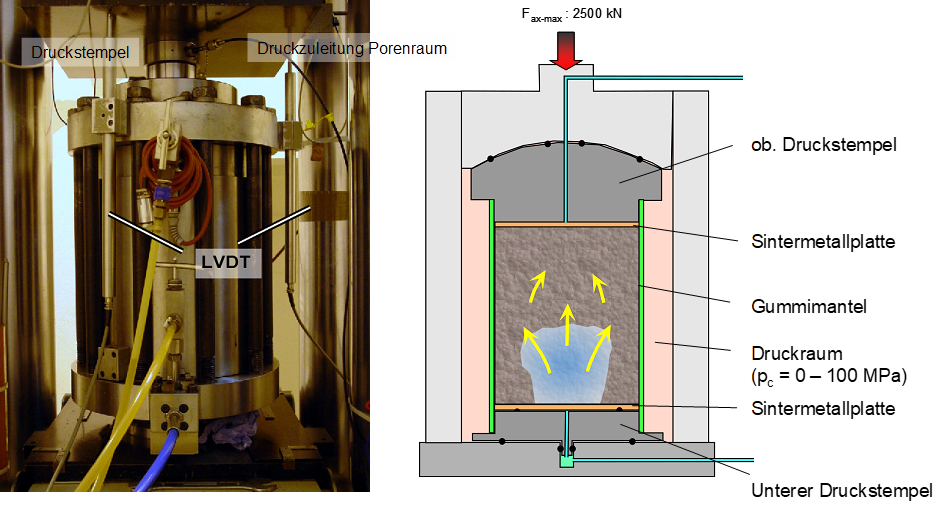
\includegraphics[width=1\textwidth]{./figures/ifg-lab-photo4.png}
\caption{Triaxial IfG pressure cell for flow tests with brine or gas.}
\label{fig:ifglabph4}
\end{figure}

The measuring principle for permeability determination under stationary conditions is based on the measurement of the flow rate $q$, here under atmospheric conditions ($p_0$), in the axial sample direction at a predetermined pressure gradient $\Delta p = p_1 - p_2$ ($p_1$ = inlet pressure, $p_2$ = outlet pressure).

The measuring arrangement used in the triaxial cell has the following advantages over the frequently used Hassler cells, in which a cylindrical sample is firmly clamped between punches and is only subjected to radial pressure.

\begin{list}{-}{\leftmargin=1em \itemindent=0em \itemsep=0em}
\item Determination of sample deformation during hydrostatic and deviatoric pressurization
\item Use of variable sample geometries (stamp sets between 60 and 110 mm diameter are available, height up to 2 x diameter)
\item The height of the gas injection pressure is limited only by the available gas cylinder pressure (routinely max: 200 bar).
\item For higher gas pressures (up to 1000 bar), a Maximator pneumatic pressure booster is used, but this is only used for special measurements.
\end{list}

For the determination of gas permeability two methods are available:
\begin{list}{-}{\leftmargin=1em \itemindent=0em \itemsep=0.1em}
\item 1st: Injection of nitrogen at a defined injection rate within a range of min. 0.1 ml / min to max. 500 ml / min under 
measurement of the injection pressure when stationary conditions are reached with leakage of the fluid against the atmosphere.
\item 2nd: Injecting nitrogen under a defined pre-pressure and measuring the flow rate at the exit side of the sample against the atmosphere.
\end{list}

\begin{figure}[!ht]
\centering
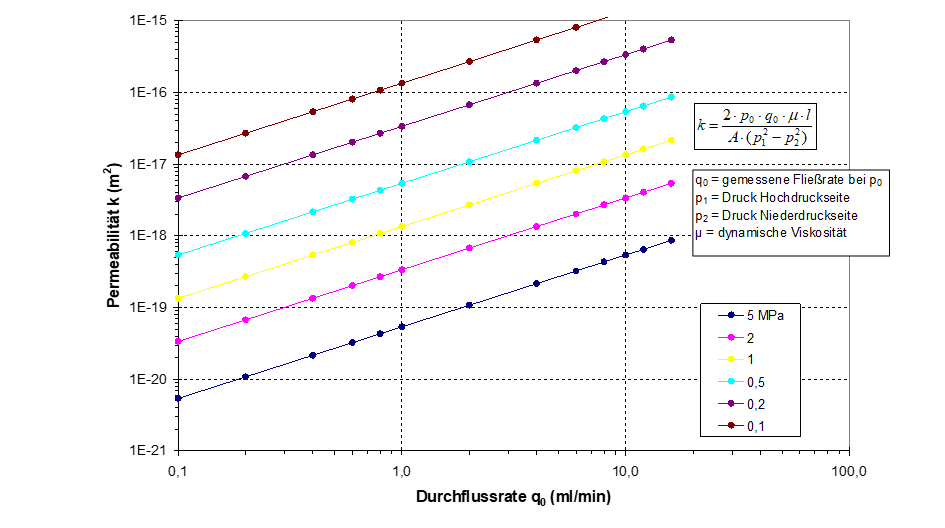
\includegraphics[width=1\textwidth]{./figures/ifg-perme-flowrate.png}
\caption{Variation diagram of permeability vs. flow rate for a sample with l = 220 mm and d = 110 mm at different injection pressures.}
\label{fig:ifgpermeflow}
\end{figure}

The lower limit of the measuring range depends essentially on the pre-pressure or the minimum measurable flow rate, as shown schematically in Fig. \ref{fig:ifgpermeflow}.
%
For gas permeability measurements, EL-FLOW mass flow controllers or flow meters from Bronkhorst are used with the following specifications:

\begin{list}{-}{\leftmargin=1em \itemindent=0em \itemsep=0em}
\item Mass flow controller Type: F-230M: Measuring range: (0) ... 10 ... 500 ml / min N2
\item Form: 200 bar / outlet pressure: 194 bar / temperature: 20$^\circ$C
\item Measuring accuracy: ± 1\% of final value, typ. better 0.5\%
\item Mass flow controller Type: F-230M: Measuring range: (0) ... 0.4 ... 20 ml / min
\end{list}

%---------------------------------------------------------------------------------------------------

\subsection{Fluid Driven Percolation Tests on Cubic Opalinus Claystone samples from Mont-Terri}
\label{sec:Percolation_Claystone_Exp}
\Authors{CAU Kiel}
\todo{Please insert authors}

The investigation of a fluid transport in claystone due to its anisotropic behavior and its role as a rock barrier in nuclear waste repositories has a great importance. Performing hydraulic fracking under pressurized fluid or storing pressurized fluids leads to the fracking of rock barrier and fluid transport through the hydraulic apertures and cavities. This can lead to pressure and volume drop in the reservoir, decrease the output and efficiency of the designed system and the contamination of ground water. In the geomechanics laboratory of CAU Kiel, the true triaxial apparatus with the maximum mechanical pressure of 600 $MPa$ and thermal loading up to 600 $^{\circ}C$ is used to conduct the fluid driven percolation in claystone samples from Mont-Terri (Figure \ref{fig:Amir_TrueTriaxial_Apparatus}). The syringe pump, with the maximum pressure of 517 $bar$, is used to pressurize the oil fluid. The cubic samples with the side dimension of 43 $mm$ and center hole length and diameter of 20 and 8 $mm$ are prepared (Figure \ref{fig:Amir_Percolation_Adapter}), respectively, and attached to the pump pipes, where the sealing is done with O-rings and epoxy glue (Figure \ref{fig:Amir_Percolation_Setup}). 

\begin{figure}[!ht]
\begin{subfigure}[c]{0.48\textwidth}
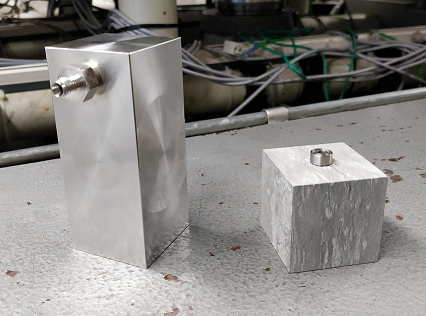
\includegraphics[width=6cm,height=4cm]{figures/Amir_Percolation_Adapter.png}
\subcaption{}
\label{fig:Amir_Percolation_Adapter}
\end{subfigure}
\hfill
\begin{subfigure}[c]{0.48\textwidth}
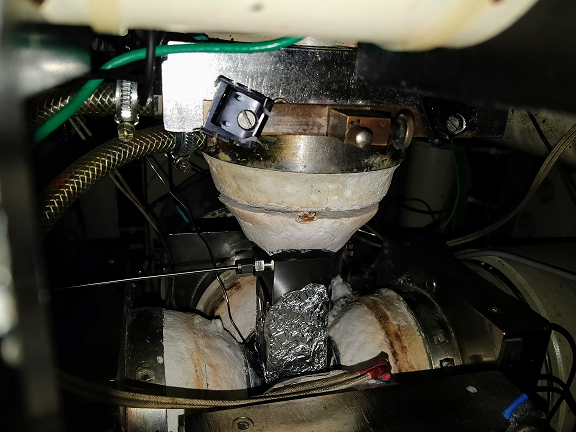
\includegraphics[width=6cm,height=4cm]{figures/Amir_Percolation_Setup.png}
\subcaption{}
\label{fig:Amir_Percolation_Setup}
\end{subfigure}
\caption{The fluid driven percolation test preparation (a) the prepared cubic claystone sample and the adapter¸ and (b) the sample placement inside the true triaxial apparatus}
\end{figure}

Two different stress configurations, as well as fluid injection directions parallel or perpendicular to the layering orientation, are considered to investigate the fracking pattern as well as flow pathways. The fracking tests are carried out under a constant fluid pressure and the peak fluid pressure, where the flow rate increases and any sudden drops in fluid pressure is recorded. In the initial test, a sample with a fluid injection direction perpendicular to the layering orientation of the Opalinus sample is considered (Figure \ref{fig:Amir_Percolation_Orientation1}). The initial stress configuration is 12, 14 and 16 $MPa$ in three different loading directions (Figure \ref{fig:Amir_Percolation_Stress_1}). In order to prevent damaging the sample prior to the hydraulic fracking test, the isotropic stresses of 8 $MPa$ is applied from all pistons and is then gradually increased to the planned stress configuration. The oil pressure is increased gradually up until the point where the borehole pressure drops and an increase in the flow rate can be seen. The test is then aborted immediately in order to avoid causing any damage to the true triaxial apparatus. In the second test setup, a sample with a fluid injection direction parallel to the layering orientation of the Opalinus sample is considered (Figure \ref{fig:Amir_Percolation_Orientation2}). The initial stress configuration is 16, 10 and 8 $MPa$ in three different loading directions (Figure \ref{fig:Amir_Percolation_Stress_2}).

\begin{figure}[!ht]
\begin{subfigure}[c]{0.48\textwidth}
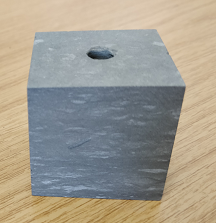
\includegraphics[width=4cm,height=4cm]{figures/Amir_Percolation_Orientation1.png}
\subcaption{}
\label{fig:Amir_Percolation_Orientation1}
\end{subfigure}
\hfill
\begin{subfigure}[c]{0.48\textwidth}
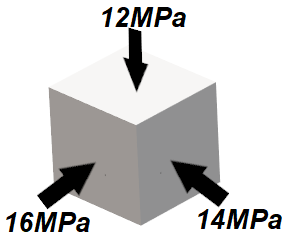
\includegraphics[width=5cm,height=4cm]{figures/Amir_Percolation_Stress_1.png}
\subcaption{}
\label{fig:Amir_Percolation_Stress_1}
\end{subfigure}
\caption{The boundary conditions for the $1^{st}$ stress configuration (a) the orientation of the embedded layers, and (b) the initial stress configuration}
\end{figure}

\begin{figure}[!ht]
\begin{subfigure}[c]{0.48\textwidth}
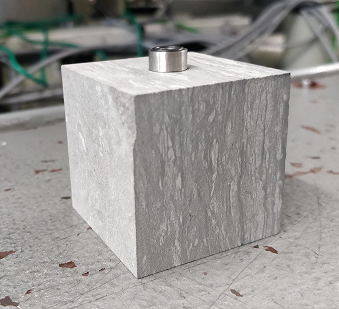
\includegraphics[width=4cm,height=4cm]{figures/Amir_Percolation_Orientation2.png}
\subcaption{}
\label{fig:Amir_Percolation_Orientation2}
\end{subfigure}
\hfill
\begin{subfigure}[c]{0.48\textwidth}
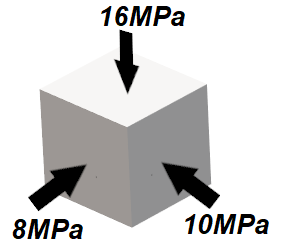
\includegraphics[width=5cm,height=4cm]{figures/Amir_Percolation_Stress_2.png}
\subcaption{}
\label{fig:Amir_Percolation_Stress_2}
\end{subfigure}
\caption{The boundary conditions for the $2^{nd}$ stress configuration  (a) the orientation of the embedded layers, and (b) the initial stress configuration}
\end{figure}

The results of the percolation tests on the Opalinus claystone samples are given in \ref{sec:mex02}, where a numerical simulation and comparison to the experimental data are provided and the effect of stress distribution, anisotropy and layering orientation on frack paths and fracking pressure are discussed. 

extra comment: change the title of 2.4.1 to be more specific (to show the difference between 2.4.1 and 2.4.2). I suggest: Pressure Driven Percolation Tests on Cylindrical Samples